\documentclass[conference]{IEEEtran}
\usepackage[english]{babel}
\usepackage{amsmath}
\usepackage{amsthm}
\usepackage{graphicx}
\usepackage[utf8]{inputenc}

%%%%%%%% SUB-FIGURE PACKAGE
\usepackage{subcaption}

%%%%%%%% HYPERREF PACKAGE
\usepackage{hyperref}
\hypersetup{linkcolor=blue}
\hypersetup{citecolor=blue}
\hypersetup{urlcolor=blue}
\hypersetup{colorlinks=true}

%%%%%%%% DEFINITION AND THEOREM DEFINITIONS
\theoremstyle{definition}
\newtheorem{definition}{Definition}[section]

\theoremstyle{remark}
\newtheorem{remark}{Remark}

\theoremstyle{remark}
\newtheorem{question}{Question}

\newtheorem{theorem}{Theorem}[section]

%%%%%%%% MULTI-COLUMNS PACKAGE
\usepackage{multicol}

%%%%%%%% BIB-LATEX STUFF
\usepackage[style=ieee,
            bibstyle=ieee,
            citestyle=ieee,
            hyperref=true,
            backend=biber]{biblatex}
\addbibresource{ref.bib} %Put relative path to ref

%%%%%%%% PERSONAL COMMANDS
\usepackage{amssymb}

%%%% Important sets
\renewcommand{\O}{\mathbb{O}}
\newcommand{\N}{\mathbb{N}}
\newcommand{\Z}{{\mathbb{Z}}}
\newcommand{\Q}{{\mathbb{Q}}}
\newcommand{\R}{{\mathbb{R}}}

%%%% Usual operations
\newcommand{\pow}[2]{#1^{#2}}
\newcommand{\expp}[1]{e^{#1}}
\newcommand{\fst}{\mathrm{fst}}
\newcommand{\snd}{\mathrm{snd}}

%%%% Lambda Calculus
\newcommand{\dneq}{\,\, \# \,\,}
\renewcommand{\S}{\pmb{\mathrm{S}}}
\newcommand{\I}{\pmb{\mathrm{I}}}
\newcommand{\K}{\pmb{\mathrm{K}}}
\newcommand{\ch}[1]{\ulcorner #1 \urcorner}

%%%% Ordinal Lambda Calculus
\newcommand{\ordAlph}{\Sigma_{\text{Ord}}}
\newcommand{\termOrd}{\text{Term}_\text{Ord}}
\newcommand{\fl}{\mathrm{fl}}
\newcommand{\sk}{\mathrm{sk}}

%% Superscript to the left
% https://latex.org/forum/viewtopic.php?t=455
\usepackage{tensor}
\newcommand{\app}[3]{\tensor*[^{#1}]{\left(#2, #3\right)}{}}

%%%% Make optional parameter
% https://tex.stackexchange.com/questions/217757/special-behavior-if-optional-argument-is-not-passed
\usepackage{xparse}

%%%% Statistics
\NewDocumentCommand{\E}{o m}{
  \IfNoValueTF{#1}
  {\mathbb{E}\left[#2\right]}
  {\mathbb{E}^{#1}\left[ #2\right]}
}
\NewDocumentCommand{\V}{o m}{
  \IfNoValueTF{#1}
  {\mathrm{Var}\left[#2\right]}
  {\mathrm{Var}^{#1}\left[ #2\right]}
}
\RenewDocumentCommand{\P}{o o m}{
  \IfNoValueTF{#1}
  {\IfNoValueTF{#2}
    {\mathrm{P}\left(#3\right)}
    {\mathrm{P}^{#2}\left(#3\right)}}
  {\IfNoValueTF{#2}
    {\mathrm{P}_{#1}\left(#3\right)}
    {\mathrm{P}_{#1}^{#2} \left(#3\right)}}
}

%%%% Lambda Calculus
\NewDocumentCommand{\cx}{o}{
  \IfNoValueTF{#1}
  {\left[\quad\right]}
  {\left[\, #1 \,\right]}
}

%%%% Create absolute value function
% https://tex.stackexchange.com/questions/43008/absolute-value-symbols
\usepackage{mathtools}
\DeclarePairedDelimiter\abs{\lvert}{\rvert}%
\DeclarePairedDelimiter\norm{\lVert}{\rVert}%
\makeatletter
\let\oldabs\abs
\def\abs{\@ifstar{\oldabs}{\oldabs*}}
%
\let\oldnorm\norm
\def\norm{\@ifstar{\oldnorm}{\oldnorm*}}
\makeatother

%%%%%%%% LOGIC TREES
\usepackage{prftree}

%%%%%%%% SPLIT EQUATIONS
% https://tex.stackexchange.com/questions/51682/is-it-possible-to-pagebreak-aligned-equations
\allowdisplaybreaks

%%%%%%%% FLOAT SPECIFIER
% https://www.overleaf.com/learn/latex/Errors/LaTeX_Error:_Unknown_float_option_%60H%27
\usepackage{float}

%%%%%%%% TO USE SHORT COMMANDS FOR VECTOR LINES
\usepackage{esvect}

%%%%%%%% ENUMERATE LABEL
% https://www.latex-tutorial.com/tutorials/lists/
\usepackage{enumitem}

%%%%%%%% DIFFERENT FONTS FOR MATH
\usepackage{mathrsfs}


\begin{document}

%%%%%% TITLE HEAD
\title{Expert System for Psychological Attention to High School Students}


\author{\IEEEauthorblockN{Juan Sebastián Cárdenas-Rodríguez}
  \IEEEauthorblockA{\textit{Department of Mathematical Science}\\
    \textit{Universidad EAFIT} \\
    Medellín, Colombia \\
    jscardenar@eafit.edu.co}}

\maketitle

\begin{abstract}
  In this work, a basic prototype for a Mamdani fuzzy inference system to detect
  depression, anxiety and hyperactivity in high school students can be found. It
  was shown that the expert system had some errors inherent from the rules
  defined. Lastly, some comparisons between some $T$-norms and defuzzification
  methods were realized.
\end{abstract}



\section{Introduction}
Mental health is crucially important for every human being and has become one of
the most important issues surrounding human health. According to the World
Health Organization\footnote{WHO's \href{https://bit.ly/34l2v94}{2001 report.}}
report of 2001, mental disorders can affect 25\% of the population, therefore,
suggesting the ongoing trend of people suffering from lack of mental health.

Furthermore, mental health is more important to monitor in adolescents and kids
as this group is in the process of developing their mental structure and
character. In this manner, as they continue creating their view about the world
they must be surrounded by a healthy environment that promotes healthy habits
and relationships with their surroundings.

As a result, schools and parents have an important responsibility to the
students of creating this environment and wisely handling mental health issues.
However, high schools do not always know how to handle or detect cases of mental
health issues. Additionally, technology has led to targeted harassing becoming
more popular over time, therefore, difficulting the probability of detecting
these cases.

Some of the most common and important mental health issues are anxiety,
depression, and hyperkinetic disorder. According to \textcite{schulte2016}, around
10\% to 20\% of children suffer from hyperkinetic disorder. Additionally, school
teachers just assume this disorder is a cause of undisciplined students and can
take the hyperkinetic student to a depressive state. These three mental
disorders can leave severe damage to a kid and can lead them to suicide.

Hence, it is of the utmost importance to quickly and efficiently detect students
that might be having a mental health issue to immediately start a process with
him/her. Furthermore, this detection has to be done with measurable variables
that can be easily obtained from questionnaires or school data.

Following the above, in this work an expert system constructed by using fuzzy
sets \parencite{zadeh1965} in a fuzzy inference system purposed by
\textcite{mamdani1981}.

\section{State of the Art}
Several expert systems to diagnose mental disorders for different groups of
people have been realized, to realize preventive diagnosis to a certain group.
The benefits of realizing this preventive diagnosis are much, as the case of the
mental disorder can be treated at the early stage and start treatment quickly.
Such is the case of the expert system developed by \textcite{nunes2009}.

According to Nunes, psychological disorders can incapacitate a worker from doing
their respective job. This occurs due to lack of an early diagnosis, as when the
disorder is detected in most cases the worker already shows signs of incapacity.
Nunes attempted to develop a hybrid expert system to make an early diagnosis of
psychological disorders.

Although Nunes's work does not present an expert system, it does highlight the
difficulty to construct one. When diagnosing a person, many factors need to be
considered such as biological data, interviews with the patient, symptoms, and
more. Furthermore, the relationship between these variables is hardly
quantifiable.

More successfully is the expert system created by \textcite{kim2006}. This
expert system uses information from psychologists, which are stored in a set of
rules that they use to diagnose a patient. The authors of that work suggest
that, although still a prototype, can become greatly elaborated with many more
clinical case studies. Furthermore, this prototype allows for non-experts to
detect cases on their children or students for the mental disorders that were
studied.

Lastly, \textcite{jabeen2018} created a cellphone application that used an
expert system to detect cases of depression and anxiety in college students.
This cellphone returned the level of sickness the student had of each mental
disorder and allowed them to ask for treatment. It is important to notice that
30\% to 35\% of students reported an abnormal level of mental disorder, highly
encouraging to further study these types of expert systems to detect these
cases.

In conclusion, although some good attempts have been realized surrounding
psychological diagnosis using expert systems, this problem is far from solved.
Each expert system has its own flaws and, therefore, it is important to continue
to build expert systems for psychological diagnosis to further improve this area
and improve people's lifestyle overall.

\section{Model}
As stated in the introduction, a Mamdani fuzzy inference system will be purposed
to solve the suggested problem. Hence, in this section the input variables of
the system, the output variables and the rules of the system will be explained.

\subsection{Input Variables}
In the first place, the first variable is the \textit{level of attention} that a
student has in class. The attention of a student can be a good indicator of
their mental health, as students with mental disorders tend to have more
difficulties focusing in class. Furthermore, specially hyperkinetic disorders
present lower attention levels than people with no disorder.

There have been several different investigations surrounding how to measure
engagement or attention, such as \textcite{wang2014}. For simplicity, this work
will measure the level of attention in the range $[0, 5]$. It is acknowledged
that this range is not strongly based on any literature but as this work focus
is the expert system, it is considered to be fitting.

There will be three different categorical values for this input low, average and
high. The low value is defined by a $\mathrm{sigmoid}$ function with parameters
$a=-5$, $c=1.7$ and $\mathrm{limit} = 0$. The average value is defined by a
$\mathrm{gauss}$ function with parameters $\mathrm{center}=2.5$ and
$\sigma = 0.7$. Lastly, the high value is defined by a $\mathrm{sigmoid}$
function with parameters $a = 5$, $c=3.3$ and $\mathrm{limit} = 5$. Each
membership function can be found in Figure~\ref{fig:att_mf}.

\begin{figure}[t]
  \centering
  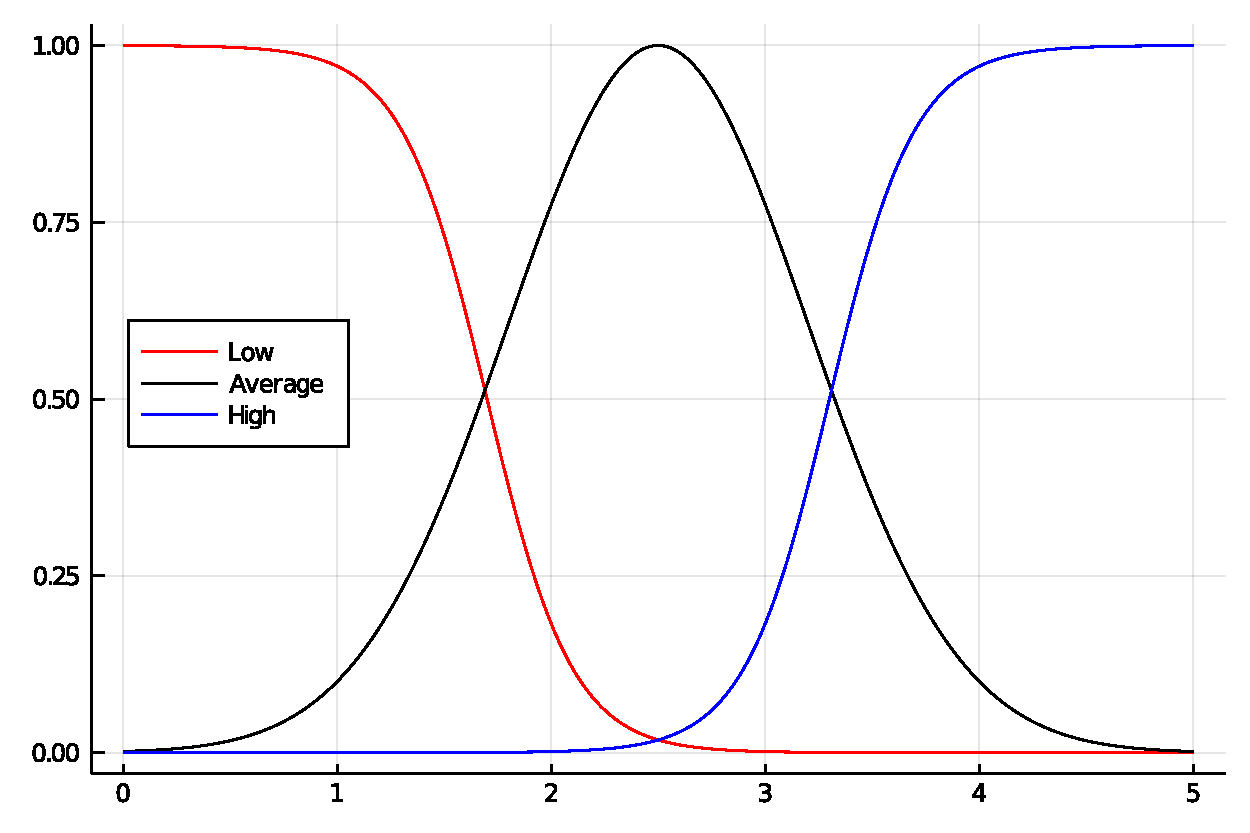
\includegraphics[scale=.3]{figs/att.pdf}
  \caption{Membership functions for the level of attention in class.}
  \label{fig:att_mf}
\end{figure}

In the second place, the \textit{academic performance} of the student will be
used as input. This input was selected as someone with low grades can lead the
student to feel depressed and have anxiety. Furthermore, excellent academic
performance can also induce anxiety on the student if pressured by parents.

The academic performance will be measured as the average of the grade of the
student. For this work, academic performance will be measured between $[0, 5]$
but it can be adjusted depending on the grading system.

Similarly to the first input, the same three categorical values will be
selected. The low value is defined by a $\mathrm{bell}$ function with parameters
$a=1.5$, $b = 4$ and $c=0$. The average value is defined by a $\mathrm{gauss}$
function with parameters $\mathrm{center}=3$ and $\sigma = 0.7$. Lastly, the
high value is defined by a $\mathrm{bell}$ function with parameters $a = 1$,
$b=4$ and $c=5$. Each membership function can be found in
Figure~\ref{fig:ap_mf}.

\begin{figure}[t]
  \centering
  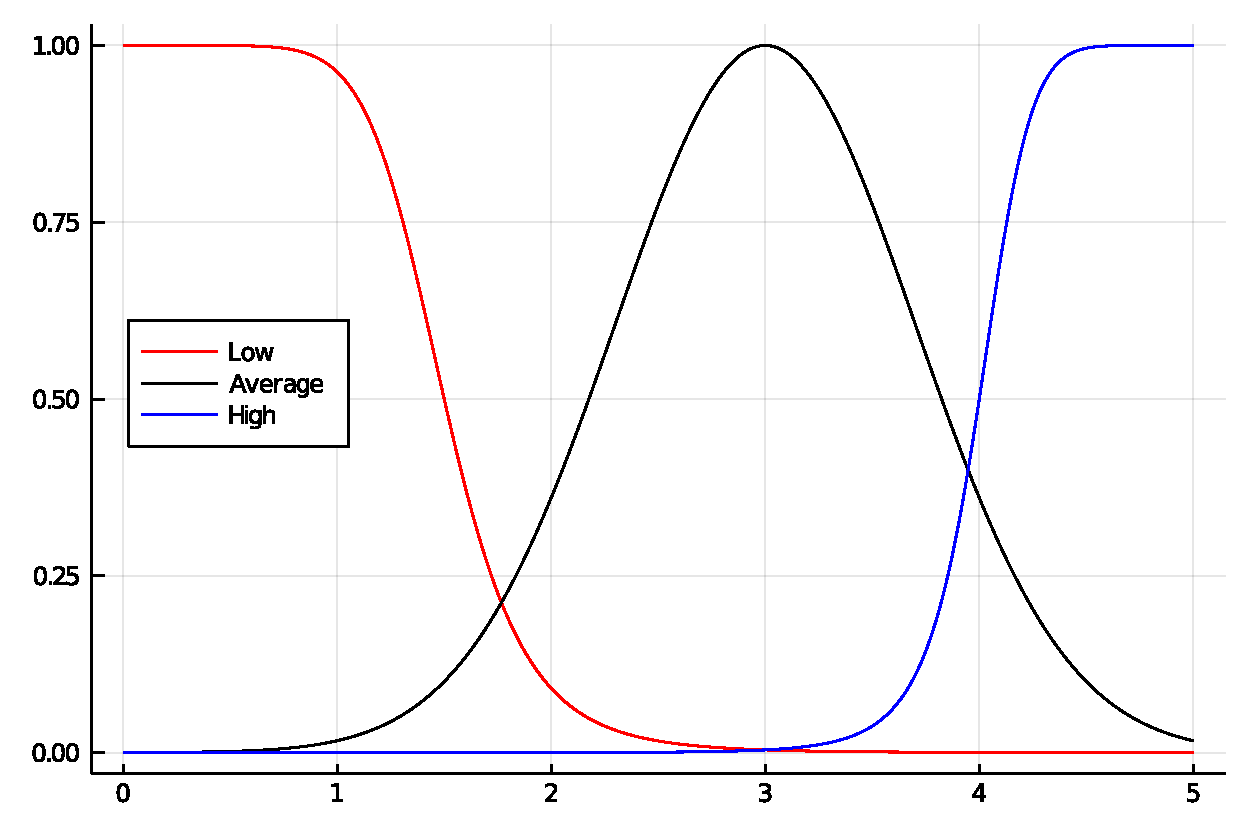
\includegraphics[scale=.3]{figs/ap.pdf}
  \caption{Membership functions for the academic performance.}
  \label{fig:ap_mf}
\end{figure}

Lastly, the \textit{emotional socialization} will be considered. As expressed by
\textcite{horner2013}, emotional socialization is one of the key features that
can determine the student's psychological health. Positively reaffirmed students
with their negative emotions can often have the best deal with feelings such as
anger, sadness, and more. Furthermore, this variable can be measured by
questionnaires to parents that would allow detecting a case easily.

The emotional socialization will be measured between $[-252, 252]$. This range
was selected based on the test done by \textcite{fabes2001} to measure emotional
socialization, as it measures positive or punitive reaffirmation of students
with this scale.

There same categorical values are chosen. The low value is defined by a
$\mathrm{sigmoid}$ function with parameters $a=-0.05$, $c=-126$ and
$\mathrm{limit} = -252$. The average value is defined by a $\mathrm{gauss}$
function with parameters $\mathrm{center}=0$ and $\sigma = 70$. Lastly, the high
value is defined by a $\mathrm{sigmoid}$ function with parameters $a = 0.05$,
$c=126$ and $\mathrm{limit} = 252$. Each membership function can be found in
Figure~\ref{fig:es_mf}.

\begin{figure}[t]
  \centering
  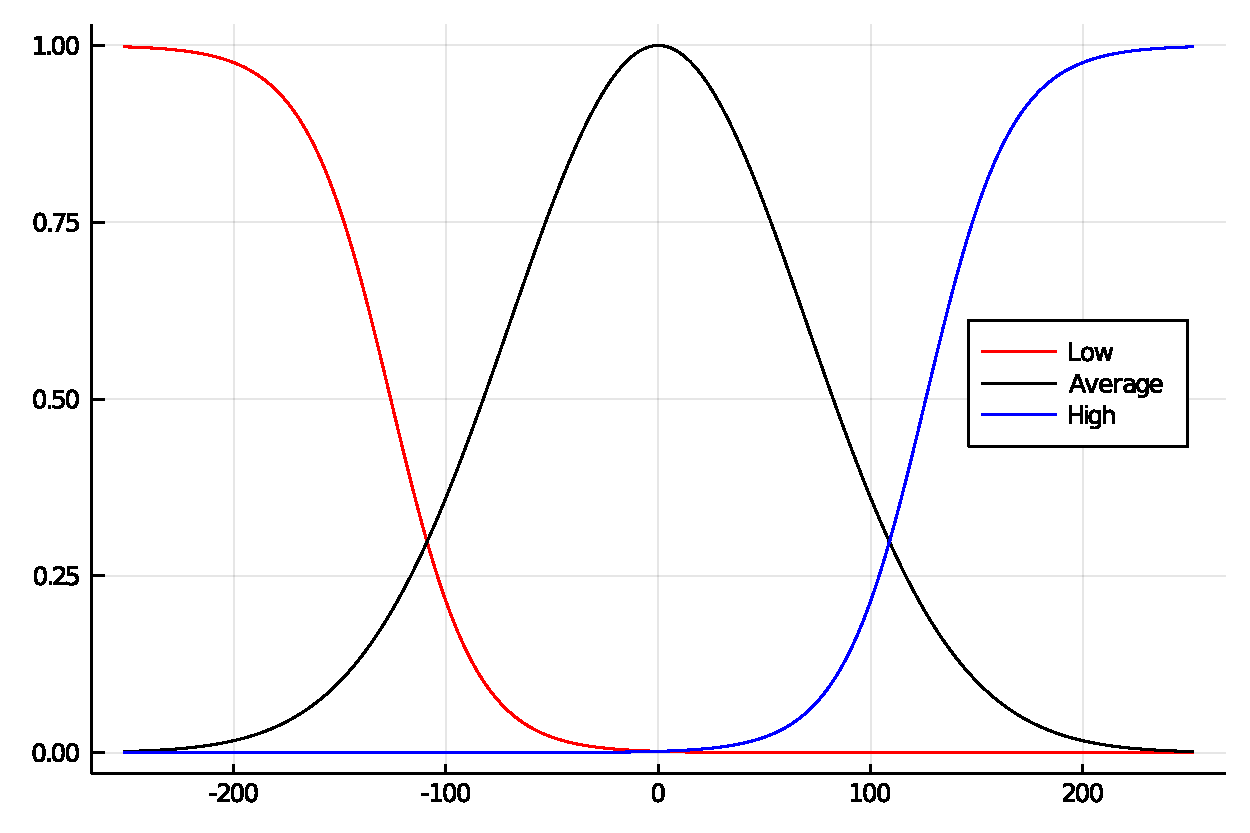
\includegraphics[scale=.3]{figs/es.pdf}
  \caption{Membership functions for the emotional socialization.}
  \label{fig:es_mf}
\end{figure}

\subsection{Output Variables}
The selected outputs are the level of \textit{depression}, \textit{anxiety} and
\textit{hyperactivity}. These three mental disorders, as explained in the
introduction, have an important role in the mental disorders presented by
students.

Each output was selected to have the same categorical values and membership
functions, to preserve simplicity. Furthermore, each output will be measured
between $[0, 100]$ to resemble a percentage of the suffering from each disease.

The two categorical values for the three outputs are low and high. The low
membership function is given by a $\mathrm{sigmoid}$ with parameters $a=-0.15$,
$c=50$ and $\mathrm{limit} = 0$. The high membership function is given by a
$\mathrm{sigmoid}$ with parameters $a=0.15$, $c=50$ and $\mathrm{limit} = 100$.
Each membership function can be found in Figure~\ref{fig:out_mf}.

\begin{figure}[t]
  \centering
  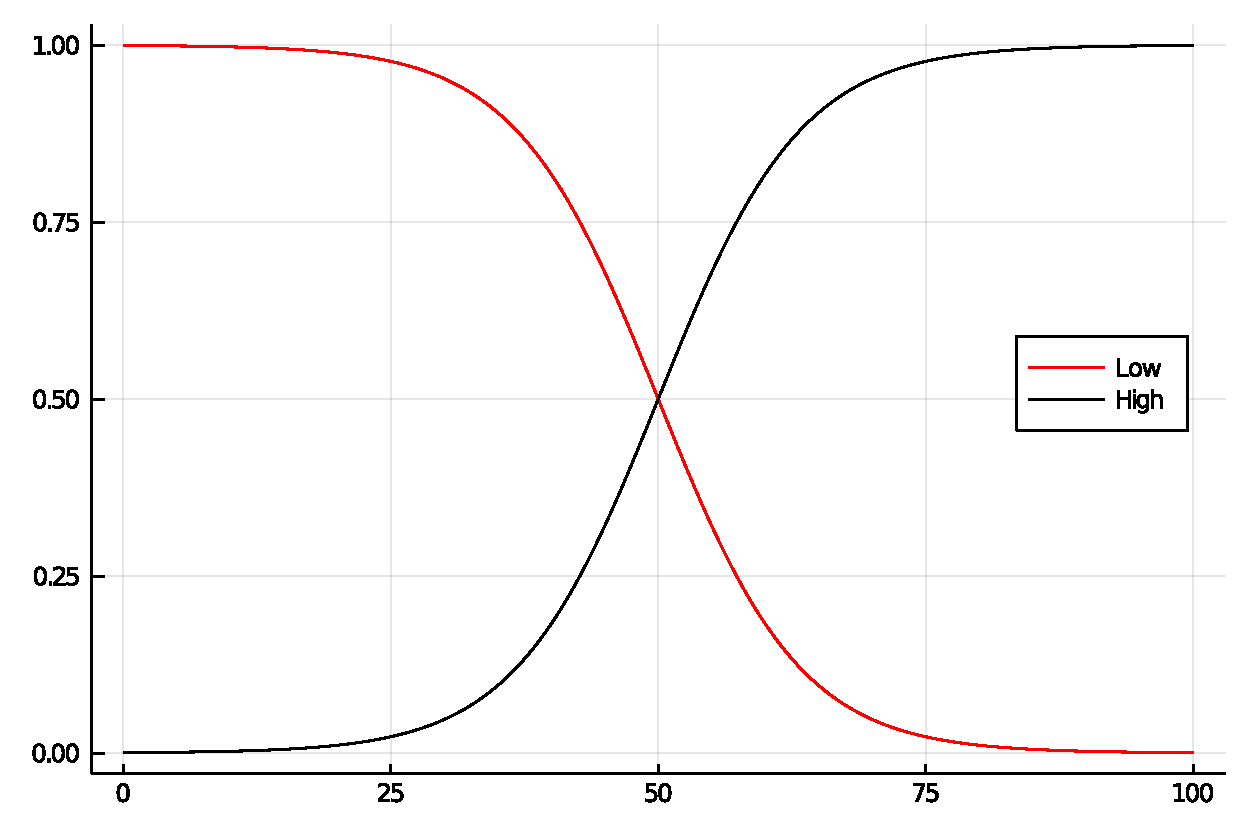
\includegraphics[scale=.3]{figs/outputs.pdf}
  \caption{Membership functions for outputs.}
  \label{fig:out_mf}
\end{figure}

\subsection{Rules}
For each rule, the level of attention will be referred as ATT, the academic
performance will be referred as AP, the emotional socialization will be referred
as ES and each of the output will be mentioned as their initial.

The rules selected are
\begin{enumerate}
  \item If the ATT is low and AP is low and ES is low then D is high and A
    is high and H is high.

  \item If the ATT is low and AP is low and ES is medium then D is high and A is
    low and H is high.

  \item If the ATT is low and AP is low and ES is high then D is low and A is
    low and H is high.

  \item If the ATT is low and the AP is medium and ES is low then D is high and
    A is low and H is high.

  \item If the ATT is low and the AP is medium and ES is medium then D is low
    and A is low and H is high.

  \item If the ATT is low and the AP is high and ES is low then D is high and A
    is low and H is high.

  \item If the ATT is low and AP is not high and ES is low then D is high and A
    is high and H is low.

  \item If the ATT is medium and AP is low and ES is low then D is high and A is
    low and H is low.

  \item If the ATT is high and the AP is low and ES is medium then D is low
    and A is low and H is high.

  \item If the ATT is high and the AP is low and ES is low then D is high and A
    is low and H is low.

  \item If the ATT is high and the AP is high and the ES is not low then D is
    low and A is high and H is low.

  \item If the ATT is high and the AP is high and the ES is high then D is low
    and A is low and H is low.

  \item If the ATT is high and the AP is not low and the ES is high then D is
    low and A is low and H is low.
\end{enumerate}

Although not every possible rule was considered, the selected set is enough to
show a prototype of this type of systems.

\section{Results}
The fuzzy inference system was implemented in the programming language
\texttt{Julia} and it was tested with the version 1.4.2. The codes can be found
annexed.

\subsection{Experiments Defuzzification}
For this set of experiments, different defuzzification methods were tested to
see the difference between them. Furthermore, for each one, the value for the
emotional socialization was fixed at -200. Additionally, this was only observed
for the depression output to make a fair comparison between them. Lastly, for
each figure, the $T$-norm is $\min$.

The first result can be seen in Figure \ref{fig:low_es}. This experiment was
observing the effect of using the weighted average defuzzification function. It
is noticed that this method, qualitatively speaking, it's the second softest
result. This is a really good property, especially comparing the computation
time that it takes to run.
\begin{figure}[t]
  \centering
  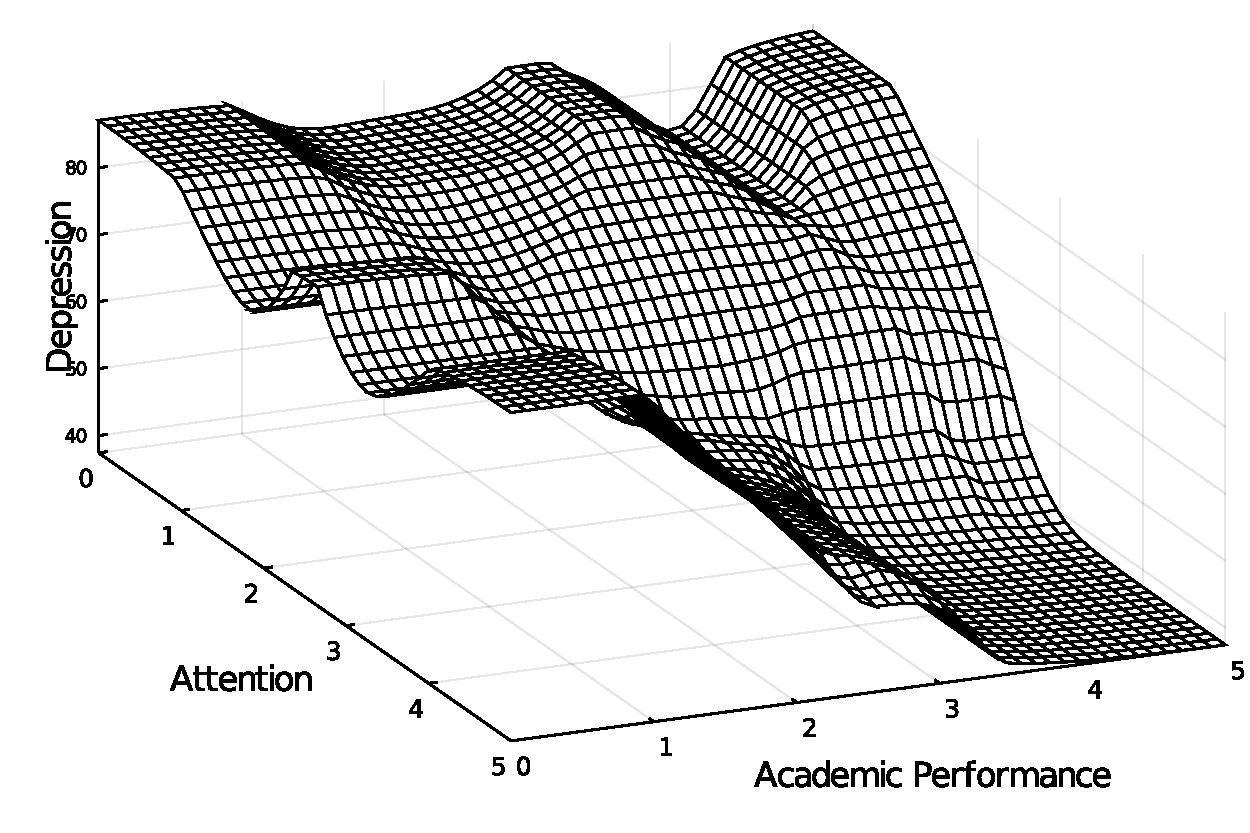
\includegraphics[scale=.3]{figs/low_es}
  \caption{Hyperplane for emotional socialization of -200 with weighted
    average.}
  \label{fig:low_es}
\end{figure}

This figure explains nicely how the variables relate to each other and confirm
that the rules partially describe correctly the desired behavior.

In the first place, it can be seen that the lowest valley for the level of
depression is seen when the attention level and academic performance is the
highest. This basic behavior has sense, as the student is having a high reward
for his attention leading him to not feel depressed.

In the second place, when the attention or academic performance is the lowest it
tends to have the biggest depression which presents a small incongruency. This
is because it is not obvious that a student with a small attention rate but a
good performance would be depressed as it's a low-risk high reward attitude. In
this manner, it is noticed that the defined set of rules have flaws.

Lastly, one of the maximum values is seen when the student has the biggest
attention but the lowest performance. This makes sense, as a student that is
constantly studying but does not perform well will feel frustration and
depression.

In Figures \ref{fig:low_es_mom}, \ref{fig:low_es_cog} the results for two more
defuzzification methods can be found. With the experiments made it is seen that
the weighted average defuzzification method was the best result at least for the
selected output.

\begin{figure}[t]
  \centering
  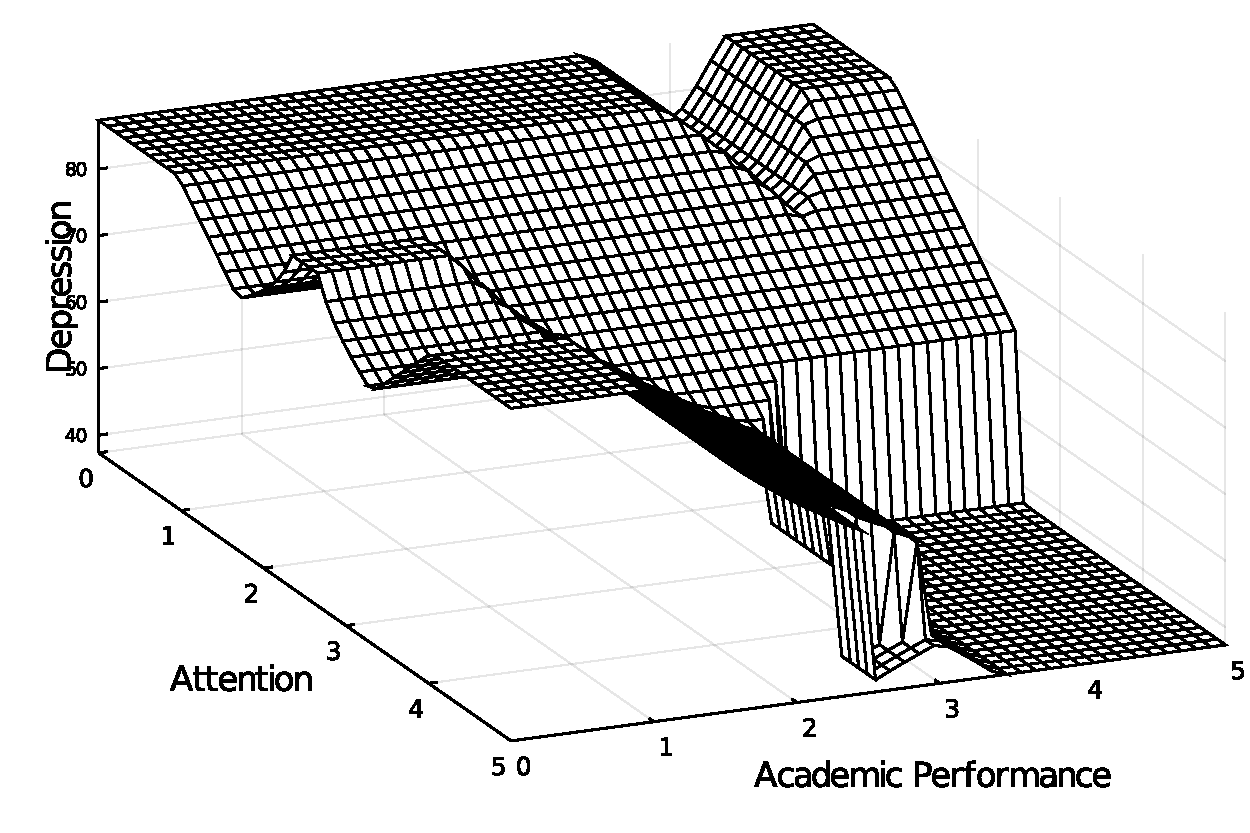
\includegraphics[scale=.3]{figs/low_es_mom}
  \caption{Hyperplane for emotional socialization of -200 with mean of maximum.}
  \label{fig:low_es_mom}
\end{figure}

\begin{figure}[t]
  \centering
  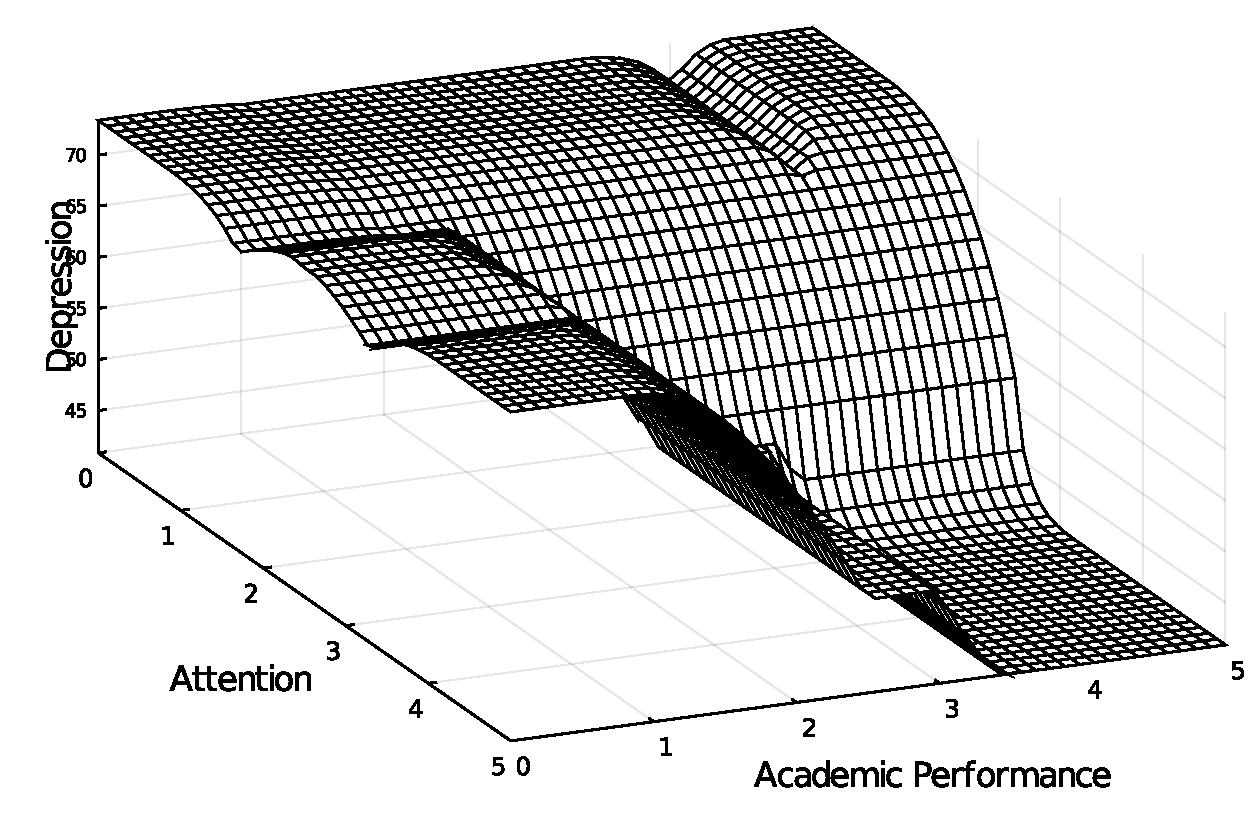
\includegraphics[scale=.3]{figs/low_es_cog}
  \caption{Hyperplane for emotional socialization of -200 with center of area.}
  \label{fig:low_es_cog}
\end{figure}

For the mean of maximum defuzzification method, it is seen that the output was
not as soft as the one obtained by weighted average. This is not a desired
behavior and, as especially in human behavior, soft curves are preferred.
However, the behavior is pretty much identical.

Lastly, for the center of area defuzzification method a softer curve was
obtained with a similar behavior. The downgrade for this method was the
computation time as, although not measured, it was significantly slower. For
further work, it is important to notice how much is the difference between those
methods to clearly decide the best option.

\subsection{Experiment T-Norm}
For this experiments, the academic performance was fixed in 5 and the weighted
average defuzzification method was used. Finally, to observe the system with
more detailed the anxiety output was selected.

\begin{figure}[t]
  \centering
  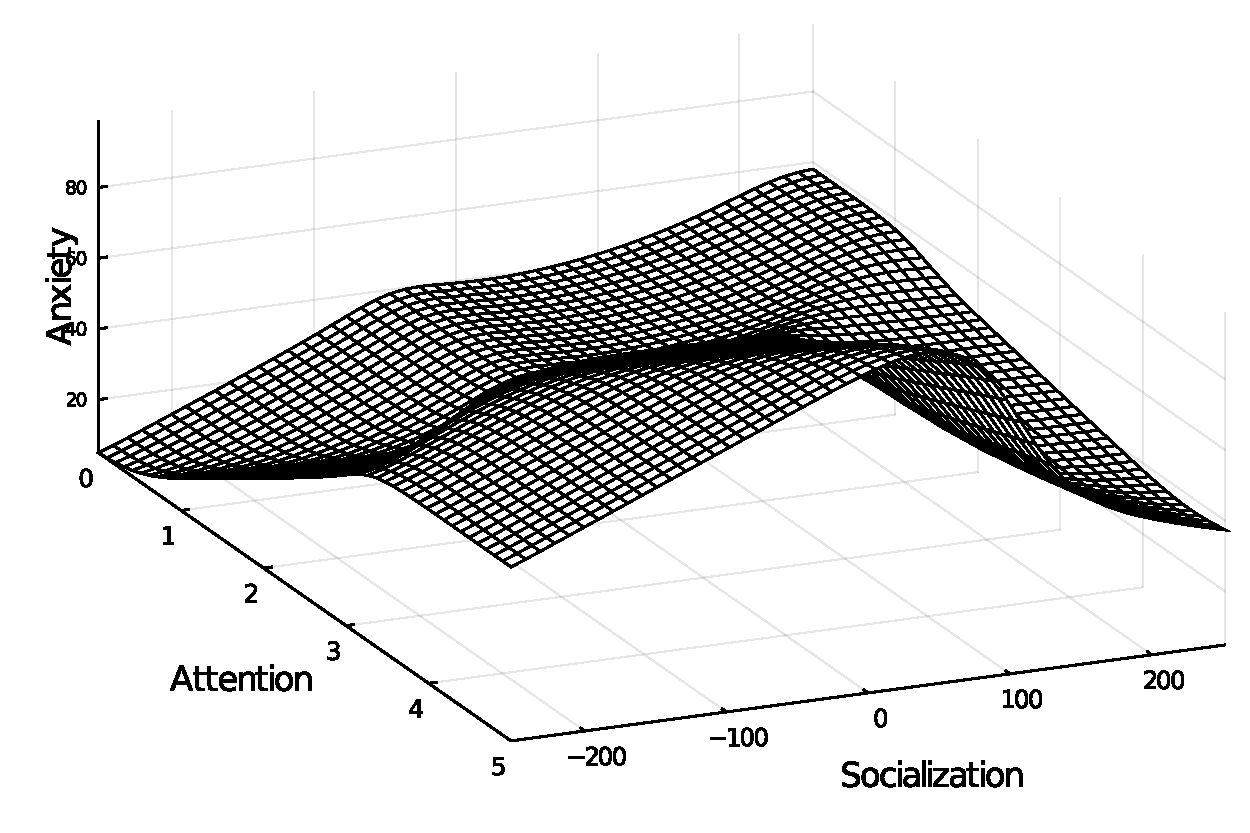
\includegraphics[scale=.3]{figs/high_ap}
  \caption{Hyperplane for academic performance of 5 using the minimum.}
  \label{fig:high_ap}
\end{figure}

\begin{figure}[t]
  \centering
  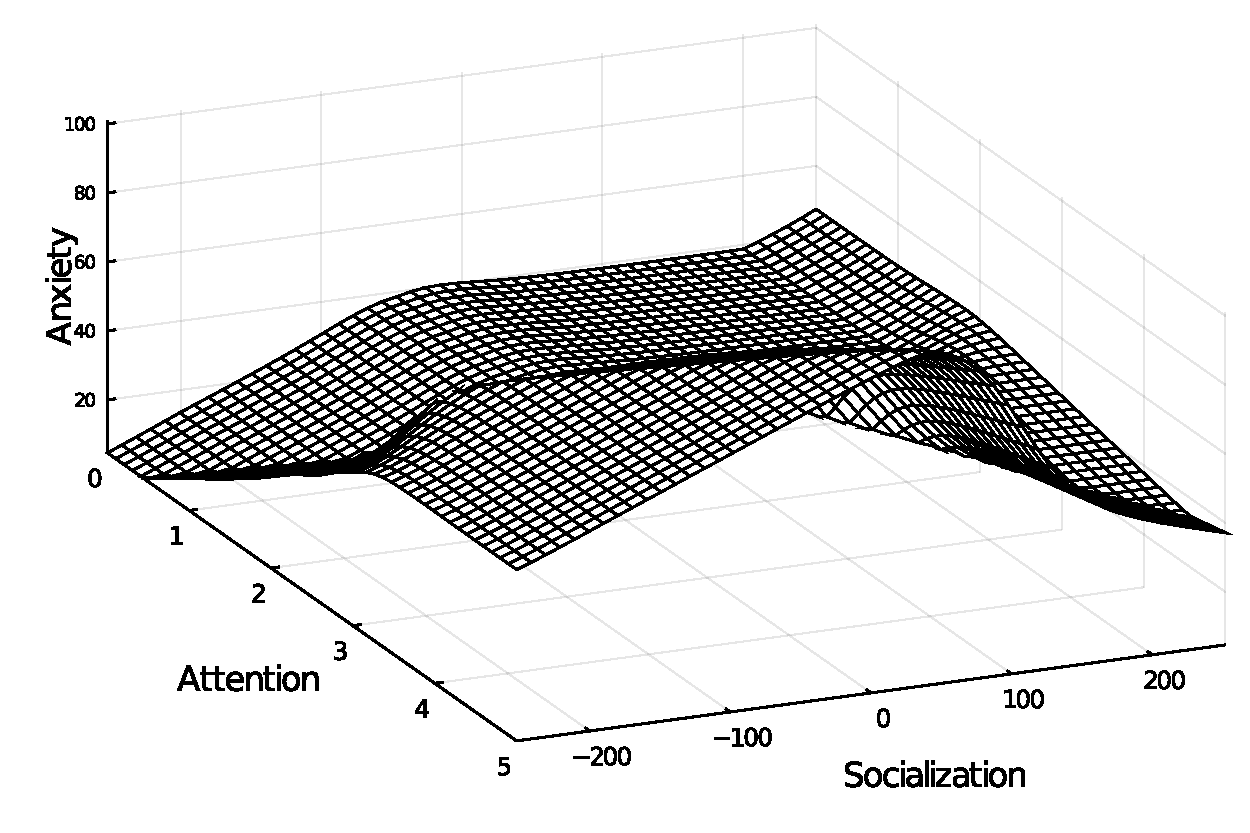
\includegraphics[scale=.3]{figs/high_ap-a-prod}
  \caption{Hyperplane for academic performance of 5 using algebraic product.}
  \label{fig:high_ap_a_prod}
\end{figure}

In Figures \ref{fig:high_ap}, \ref{fig:high_ap_a_prod} the experiments for this
section with different $T$-norms can be found. It is important to remark that it
is seen that the hyperplanes did change slightly their form, even if the fuzzy
inference system stayed the same. This highlights the importance of selection the
norm and how each one affects the outputs.

It is seen that the algebraic product does have a more softer output than the
minimum. Furthermore, although the minimum norm is bigger than the algebraic
product, that inequality is not preserved through the output as seen in
$(0, 200)$ point. This is important to notice as selecting a bigger norm does
not imply a bigger output.

Lastly, it is stated that the surface does not reflect the desire behavior. In
first glance, a student with small attention span and high socialization should
not have that much anxiety. Therefore, as shown in the previous experiments, the
fuzzy inference system purposed has some incoherent behavior and it is not ready
to take expert decisions.

\section{Conclusion}
In conclusion, a basic prototype for a Mamdani fuzzy inference system was
constructed. This fuzzy inference system presents some incoherent behavior but
has partially some good outputs. This reinforces the idea that tackling this
problem from this angle can be done but it does has some complexities hard to
represent.

Furthermore, a comparison between $T$-norms and defuzzification methods was
realized, which showed some of the incongruities. Additionally, it allowed to
compare between the outputs in which the best defuzzification method used was
the weighted average as it was the fastest one with a good semi-soft curvature.

\printbibliography
\end{document}


